\documentclass[11pt, oneside]{report}
\usepackage[a4paper,top=3cm,bottom=3cm,left=3cm,right=2cm]{geometry}
\usepackage[utf8]{inputenc}
\usepackage[T1]{fontenc}
\usepackage{graphicx}
\usepackage{url}
\usepackage{float}
\usepackage{titlesec}

\usepackage[hidelinks,breaklinks]{hyperref}
\usepackage[slovak]{babel} % vypnite pre prace v anglictine
\usepackage{listings}\usepackage{graphicx}
\graphicspath{ {images/} }

\usepackage{color}
\definecolor{gray}{rgb}{0.4,0.4,0.4}
\definecolor{darkblue}{rgb}{0.0,0.0,0.6}
\definecolor{cyan}{rgb}{0.0,0.6,0.6}
\definecolor{orange}{rgb}{1,0.45,0}

\lstset{
  basicstyle=\ttfamily,
  columns=fullflexible,
  showstringspaces=false,
  commentstyle=\color{gray}\upshape
}

\lstdefinelanguage{XML}
{
  morestring=[b]",
  morestring=[s]{>}{<},
  morecomment=[s]{<?}{?>},
  stringstyle=\color{black},
  identifierstyle=\color{darkblue},
  keywordstyle=\color{cyan},
  morekeywords={xmlns,version,type}% list your attributes here
}

\lstdefinelanguage{JavaScript}{
  morekeywords={typeof, new, true, false, catch, function, return, null, catch, switch, var, if, in, while, do, else, case, break},
  morecomment=[s]{/*}{*/},
  morecomment=[l]//,
  morestring=[b]",
  morestring=[b]'
}

\lstdefinelanguage{HTML5}{
		showstringspaces=true,
		keepspaces=true,
        language=html,
        sensitive=true, 
		literate=%
		{@}{{{\color{orange}@}}}1
		{\{}{{{\color{orange}\{}}}1
		{\}}{{{\color{orange}\}}}}1,
        alsoletter={<>=-},
        otherkeywords={
        % HTML tags
        <html>, <head>, <title>, </title>, <meta, />, </head>, <body>,
        <canvas, \/canvas>, <script>, </script>, </body>, </html>, <!, html>, <style>, </style>, ><
        },
        ndkeywords={
        % General
        =,
        % HTML attributes
        charset=, id=, width=, height=,
        % CSS properties
        border:, transform:, -moz-transform:, transition-duration:, transition-property:, transition-timing-function:
        },  
        morecomment=[s]{<!--}{-->},
        tag=[s],        
}

\usepackage[backend=bibtex,
                style=authoryear,
                natbib=true, 
                style=numeric-comp
                ]{biblatex} 
\DeclareFieldFormat{url}{\url{#1}}
\bibliography{literatura.bib} 
\linespread{1.2} % hodnota 1.25 by mala zodpovedat 1.5 riadkovaniu
\pagenumbering{arabic} 
\urlstyle{same}

\titleformat{\chapter}{\normalfont\huge\bf}{\thechapter.}{20pt}{\bf}
\titlespacing*{\chapter}{0pt}{0pt}{20pt}

% -----------------
% --- Definicia zakladnych pojmov
% --- Vyplnte podla vasho zadania
% -------------------
\def\mfrok{2018}
\def\mfnazov{BAKALÁRSKA PRÁCA}
\def\mfnazovprace{Odborná prax}
\def\mfautor{Michal Falát}
\def\mfskolitel{Petr Šaloun }
\def\mfkonzultant{Boros Kovař }  

\def\mfmiesto{Ostrava, \mfrok}
\def\mfodbor{2508 Informatika} 
\def\program{ Informatika }
\def\mfpracovisko{ Katedra informatiky }
\def\mftyp{bakalarka }

\begin{document}  


% -------------------
% --- Obalka ------
% -------------------
\thispagestyle{empty}

\begin{center}
\sc\large
VŠB - Technická univerzita Ostrava\\
Fakulta elektrotechniky a informatiky


\vfill

{\LARGE\mfnazov}\\
\end{center}

\vfill

{\sc\large 
\noindent \mfrok \hfill  \hfill \mfautor
}

\eject % EOP i
% --- koniec obalky ----


\thispagestyle{empty}
\noindent

\begin{center}
\sc  
\large
V\v SB - Technická univerzita Ostrava\\
Fakulta elektrotechniky a informatiky

\vfill

{\LARGE\mfnazovprace}\\
\end{center}

\vfill



{\sc\large 
\noindent \mfrok \hfill  \hfill \mfautor
}

\eject % EOP i
\setcounter{page}{3}
\newpage 


\setcounter{page}{4}

\vfill
{\bf Poďakovanie:} Chcel by som poďakovať svojim kolegom  z práce, ktorí si na mňa našli čas a boli ochotni mi pomôcť a vysvetliť akýkoľvek problém. Poďakovanie patri aj môjmu konzultantovi, Borisovi, ktorý mi zastrešil odbornú prax a venoval mi aj svoj voľný čas.

% --- Koniec poďakovania

% -------------------
%   Abstrakt - Slovensky
% -------------------
\newpage 
\section*{Abstrakt}


Táto bakalárska práca popisuje absolvovanie odbornej praxe vo firme. V prvej časti  sa  v krátkosti   vysvetľuje činnosť a  zameranie firmy M2M Solutions s.r.o, v ktorej som   vykonával prax. Ďalšia  časť je venovaná samotným projektom a  zadaniam  spolu s riešeniami, na ktorých som pracoval. V závere práce popisujem   celkový súhrn  a využitie  znalostí  nadobudnutých počas školy a technológie, ktoré  som sa musel individuálne doučiť.



\paragraph*{Kľúčové slová:} ASP.NET, Java, Angular, Typescript, MVC
% --- Koniec Abstrakt - Slovensky

\paragraph*{}

\section*{Abstract}
This bachelor thesis describes my individual practise in company. In first section I explain the company  M2M Solutions s.r.o,its activities and products. Next section is dedicated to tasks and solutions, which I work on. Finally I explain sumary of practise and usage of technologies, that a learn during school and technologies which I have to learn on my own.


\paragraph*{Keywords:}  ASP.NET, Java, Angular, Typescript, MVC
% --- Koniec Abstrakt - Anglicky


%prehlasenie

% -------------------
% --- Obsah
% -------------------

\newpage 
\tableofcontents

% ---  Koniec Obsahu

% -------------------
% --- Zoznamy tabuliek, obrázkov - nepovinne
% -------------------

\newpage

\chapter*{ Zoznam symbolov a skratiek }
\addcontentsline{toc}{chapter}{Zoznam skratiek}  
\begin{table}[H]
\label{my-label}
\begin{tabular}{lllll}
API  & - &  application programming interface &  &  \\
ASP&- &Active Server Pages  &  &  \\
HTML & - &  Hypertext Markup Language&  &  \\
JS   & - & Javascript  &  &  \\
JSON & - & Javascript object notation &  &  \\
MVC  & - &  Model View Controller &  &  \\
NF & - &  Normálna forma &  &  \\
RSS & - &  Rich Site Summary &  &  \\
SQL  & - &  Structured Query Language&  &  \\
SPA  & - &  Single Page application&  &  \\
XML  & - &  eXtensible Markup Language &  &  \\
 &  &  &  &  \\
 &  &  &  & 
\end{tabular}
\end{table}
\newpage 

\listoffigures
%\chapter{Zoznam Obrázkov}
\addcontentsline{toc}{chapter}{\listfigurename}

\newpage 

\listoftables
\addcontentsline{toc}{chapter}{\listtablename}

% ---  Koniec Zoznamov



%\chapter{Úvod}
\input uvod.tex 

\input firma.tex

\chapter{Popis projektov}
\section{Multimediálne informačné panely}
Multimediálne informačné panely\cite{panely} je webová aplikácia napísaná v ASP.NET s MVC architektúrou. Je využívaná na zobrazovanie rôznych  informácii na obrazovkách v rôznych časových slotoch. Aplikácia má  možnosť  jednoducho pridávať a meniť obsah  jednotlivých stránok, ktoré sa zobrazujú na obrazovkách.  Správanie a obsah stránok môže byť podla potreby nastavený pre každý panel samostatne. Vďaka tomu má široké využitie najmä  vo výrobe v logistike či v obchodných centrách.
\section{LightNet TK}
LightNet TK je webová aplikácia (Tenký klient), ktorá slúži na zobrazovanie dôležitých informácii o verejnom osvetlení pre starostov obcí. Jedná sa hlavne o zobrazovanie porúch vzniknutých na rozvádzačoch, časy svietenia jednotlivých lámp, mapy a iné dôležié informácie. Hierarchia systému sa  skladá z 2 častí:
\begin{itemize}
\item Aplikačné rozhranie (API) napísané v jazyku Java s použitím technológie Spring Boot
\item Webový klient - SPA aplikácia, ktorá komunikuje s API. Je napísaná v Typescripte s použitím framweorku Angular
\end{itemize} 

\section{.NET platforma M2Ms}
.NET platforma M2Ms - Tvorí jadro, ktoré je použité v každom projekte .NET. Jej vývoj začal v máji 2017 a v súčasnosti sa  M2Ms .NET platforma je komponentovo orientovaná a propietárne vyvintá .NET tímom  vo  firme M2M solutions. Je v poradí 3. platforma Narozdiel od minulých verzii, ktoré fungovali na ASP WebForms, nová platforma beží na MVC5,
%M2Ms IoT - je pomerne malá časť rozsiahleho projektu, ktorý vynikol na základe požiadavky pre použitie IoT vo výrobnej hale. Jedná sa o android mobilnú aplikáciu, ktorá slúži ako kontroler medzi bezdrôtovými tlačidlami zn. Flic\cite{flic} a webovým rozhraním, ktoré zachytáva jednotlivé udalosti a robí ďalšiu business logiku. Každá udalosť vyvolaná tlačidlom, je vložená do fronty v mobilnom zariadení(SQL Lite databáza)  a následne poslaná na rozhranie. V prípade neúspešného odoslania ( napr. výpadok siete, nedostupnosť serveru a pod. )   je možné zadefinovať interval pre  opätovný pokus odoslať všetky neúspešné udalosti z fronty na rozhranie.

\chapter{Použité technológie}
V tejto sekcii v krátkosti zhrniem základné informácie o technológiach, s ktorými som sa počas odbornej praxe stretol a aktívne využíval. Okrem týchto  technológii som samozrejme používal radu ďalších, ale v menšej miere.

\section{.NET Framework}

.NET framework \cite{net} je bezplatná platforma vyvíjaná spoločnosťou Microsoft. Prvýkrát bola predstavená ešte v roku 2002 pod názvom .NET Framework 1.0. V súčasnosti sa používa verzia .NET 4.7, ktorá bola vydaná v roku 2017. Táto platforma obsahuje veľké množstvo knižníc napríklad pre prácu   so sieťou, s grafikou,  so súbormi a podobne. Je určená pre vývoj rôznych typov aplikácii. S pomocou .NET  je možno jednoducho vytvoriť napríklad webovú, mobilnú alebo desktop aplikáciu. Ďalšou veľkou výhodou tohto frameworku je, že je možné  s ním racovať vo viacerých programovacích jazykoch ako napr Visual Basic, F\# alebo najpoužívanejší C\#. Pre rozšírenie funkčnosti aplikácie je možnosť pridať ďalšie knižnice, ktoré sú ľahko stiahnutelné cez NuGet package manager. Počas praxe som využíval hlavne ASP.NET, ktorý je určený na vývoj webových stránok.

\section{Angular}
Angular\cite{angular} ( Často označovaný aj ako Angular2) je multiplatformový  open-source webový framework, v ktorom sa vyvíja front-end časť aplikácie. Pôvodne bol vyvinutý firmou Google v roku 2010 pod názvom AngularJS. Pre jeho obľúbenosť a široké  možnosti použitia bol koncom roka 2016 vydaný úplne nový framework Angular, ktorý s pôvodným AngularJS nemá už nič spoločné. V súčasnosti sa používa najnovšia verzia Angular 5.2.0.
Jeho veľkou výhodou je používanie jazyku Typescript od firmy Microsoft,  s ktorým je možné vytvárať triedy, rozhrania a podporuje dátové typy, čo bežný Javascript nepodporuje. Angular disponuje dostatočným počtom knižníc a komponentov pre vývoj  SPA webovej aplikácie. Pre užívateľské rozhranie a príjemný UX zážitok je možné pridať aj knižnicu Material design \cite{material}, s ktorou  sa aplikácia stane moderná, prehľadná a responzívna.

\section{GIT}
GIT\cite{git} je distribuovaný systém na správu verzií. Bol vytvorený Linusom Torvaldsom v roku 2005. Pôvodne bol určený pre správu jadra operačného systému Linux. Jeho výhodou je, že každý užívateľ má vlastný repozitár, v ktorom môže robiť lokálne zmeny (príkaz \textit{commit}). Tieto zmeny môže následne zosynchronizovať  so serverom ( príkazy \textit{ pull, push}). Pri riešení konfliktov medzi lokálnzm repozitárom a serverom je použitý trojcestný zlučovací algoritmus (\textit{3-way merge}) 

\chapter{Zadané úlohy a riešenia}
\section{Multimediálne informačné panely}
Na tomto projekte som pracoval  priebežne počas  obidvoch semestrov. Jednalo sa najmä o  odstraňovanie existujúcich chýb nahlásených zákazníkmi (Bugfixing), ale aj o vytváranie ďalších komponentov a úpravu podľa požiadaviek. Práca na tomto projekte pozostávala z 3 väčších úloh  a  niekoľkých menších úloh(upravenie niektorých prvkov na stránke, zmeniť umiestnenie tlačidiel, preklad užívateľského manuálu do anglického jazyka a podobne)
\subsection*{Komponent RSS čítačka}
\textit{Zadanie:}\\
Pridať do projektu  komponent na zobrazenie obsahu z ľubovolného RSS zdroja a vytvoriť formulár na jeho editáciu.
\\\textit{Analýza:}\\
 RSS zdroj   je určený na čítanie noviniek  z webových stránok ako napríklad spravodajstvo, počasie, kurzové meny a pod. Takéto informácie  z internetu si na multimediálnych informačných paneloch nájdu svoje uplatnenie. Mojou úlohou bolo naimplementovať komponent RSS čítačka, pridať  konfigurovatelné nastavenia pre tento komponent a otestovať jeho funkčnosť.
Všetky ostatné komponenty sú implementované ako súbor JS funkcií s niekoľkými riadkami HTML kódu. Samotné ukladanie komponentov v databáze je riešené veľmi netradične. Jednotlivé komponenty nie sú ukladané ako konkrétne záznamy v tabuľke, ale celá stránka  so všetkými svojimi komponentami vrátanie JS a HTML je uložená ako jeden textový stĺpec. Toto nešťastné riešenie  pochádza  zo začiatkov pôsobenia firmy, kedy sa ešte nebral veľký ohľad na  škálovatelnosť a  správnosť ukladania dát. 
Napriek tomu, že je porušený 1NF a 2NF, je produkt plne funkčný a používaný aj v súčasnosti. V rámci zachovania tohto konceptu som sa rozhodol pokračovať rovnakým spôsobom ukladania komponentov do databázy.
\\\textit{Riešenie:}\\
Ďalšia časť spočívala v naštudovaní samotného fungovania zobrazovania RSS zdroja. RSS feed je v podstate pravidelne upravovaný XML súbor, ktorý je možné stiahnúť z nejakého servera. V samotnom XML dokumente môžeme nájsť RSS verziu (V súčasnosti sa používa verzia 2.0 ) Dokument pozostáva z niekoľkých ďalších uzlov ako \lstset{language=XML}
\lstinline!<title> , <description>, <link>!. Posielanie dotazu na RSS zdroj priamo z javascriptovej funkcie nebolo možne kvôli cross origin právam -t eda posielanie  dotazov na inú deménu. To som obišiel vypnutím v súbore web.config. V javascripte sa už iba dotazujem na funkciu z kontrolleru, ktorá  už dokáže pristupovať aj k veciam  na inej doméne. Na editáciu som puužil jQuery UI dialóg, ktorý používame v celom projekte. Do editora som sa rozhodol vložiť polia na URL adresu zdroja a niekoľko checkboxov. Tieto checkboxy dokážu napríklad skryť jednotlivé  uzly,  pohybovať text, skryť hlavičky uzlov. Ďalej som pridal polia na limit uzlov items, keďze niektoré zdroje môžu obsahovať veľmi veľa týchto uzlov aj keď užívateš potrebuje napríklad prvé 3 uzly. Nakoniec editora som pridal textové pole na zadanie onbovovacieho intervalu v minútach. Tento údaj vyjadruje, v akom inteervale bude vykonaný dotaz na náš RSS zdroj. Pre zadanie číselných údajov som sa rozhodol použiť jeden z nových atribútov  v HTML5 pre elimináciu zadania písmen a iných znakov:
\begin{center}
\lstset{language=HTML5}
\lstinline!<input type="number" value="0" id="refreshRSS@{compId}">!\\
\end{center}
V ukážke je použitá aj Razor syntax. Razor je  akási nadstavba pre ASP.NET , pomocou ktorej je možné upravovať HTML stránky pomocou syntaxe z C\#. V Razore  sa môžu použiť cykly, podmienky, modely, ale aj rôzne iné veci, ktoré potrebujeme. V tomto prípade je potrebné jednoznačne identifikovať, pre ktorý RSS komponent robíme úpravy. Identifikátor komponentu je uložený v premennej \textsf{@\{compId\}}.\\
Po prijatí RSS feedu ostávalo prejsť všetky uzly v dokumente a podľa parametrov v editore  zobraziť potrebné údaje. Na prechádzanie  XML štruktúry som sa rozhodol použiť zabudovaný nástroj jQuery, kde pomocou funkcie 
\lstset{language=Javascript}
\lstinline!jQuery.parseXML(data)!
vieme previesť  do štruktúry, kde môžeme jednoducho  dostať potrebné uzly, ich dáta, prípadne atribúty. Na záver už pstávalo iba skontrolovať inerval dotazovania a doladiť zobrazovanie  dát.
\begin{figure}[h]
    \centering
    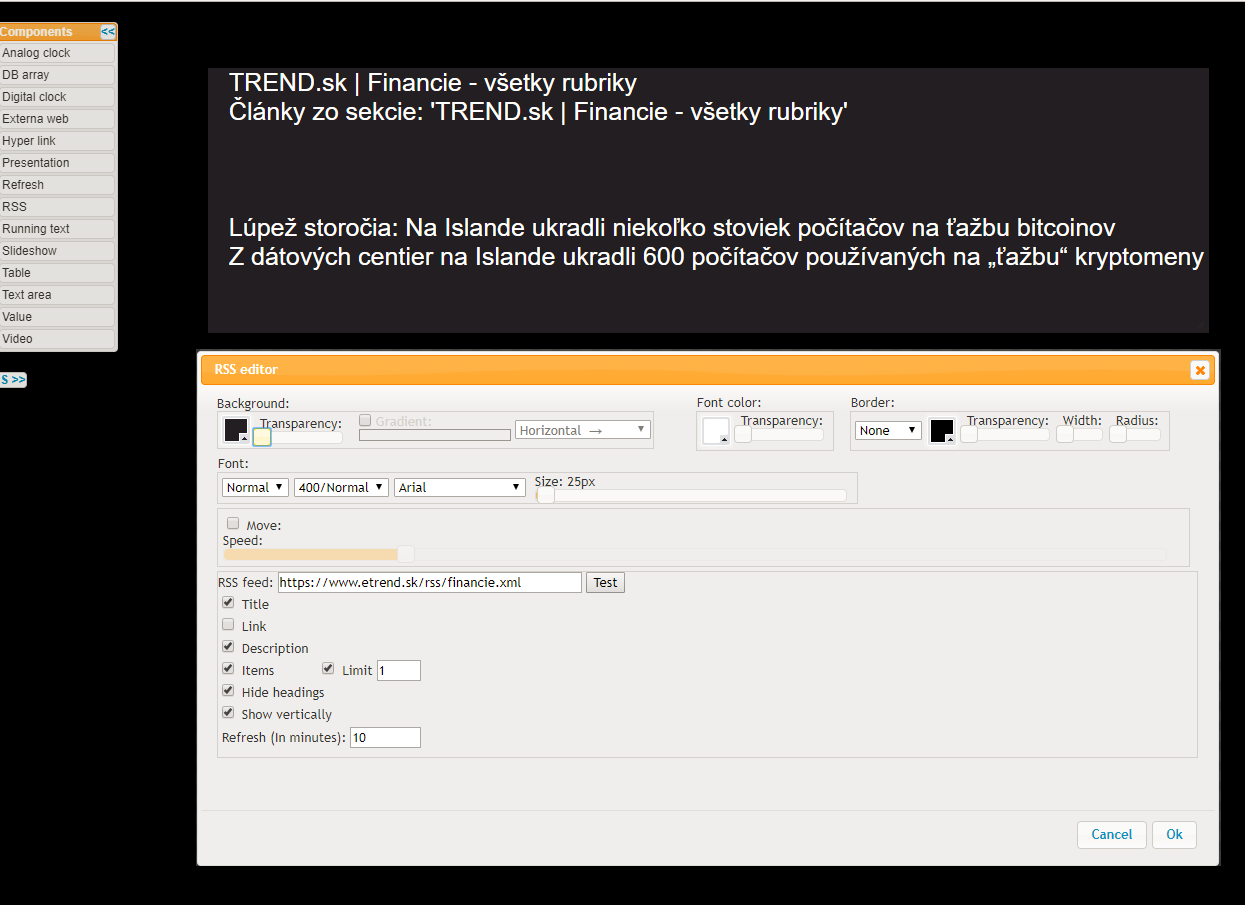
\includegraphics[width=0.85\textwidth]{RSS}
    \caption{Ukážka editora(Dole) a RSS obsahu (Hore)}
    \label{fig:mesh1}
\end{figure}

\subsection*{Pridanie užívateľských rolí}
\textit{Zadanie:}\\
Upraviť bezpečnosť chodu aplikácie pridaním užívateľských rolí a overiť ich funkčnosť.
\begin{enumerate}
\item \textbf{Administrátor} - má možnosť pridať/editovať/vymazať panel, má možnosť pridať/editovať/vymazať stránku, má prístup k nastaveniam, môže manipulovať s časovou osou.
\item \textbf{Autor} - má možnosť pridať/editovať panel, nemôže vymazať žiadny panel, má možnosť pridať/editovať/vymazať stránku, nemá prístup k nastaveniam, môže manipulovať s časovou osou.
\item \textbf{Bežný používateľ} - nemá možnosť pridať/editovať/vymazať panel, nemá možnosť pridať/editovať/vymazať stránku, nemá prístup k nastaveniam, nemôže manipulovať s časovou osou.
\end{enumerate}
\textit{Analýza}\\
Táto požiadavka prišla od zákazníka, ktorý chcel takýmto spôsobom zvýšiť bezpečnosť chdu aplíkácie.
V prvej časti budeme musieť upraviť tabuľku \textsf{users} a pridať do nej stĺpec, ktorý nám bude vyjadrovať konkrétnu užívateľskú rolu. V ďalšej časti, bude potrebné prejsť všetky stránky a kontrollery a upraviť ich podľa zadania. 
\textit{Riešenie}\\
Postup je rozdelený do viacerých krokov. V prvom kroku budeme musieť upraviť DB model v kóde aj  pridať stĺpec do databázy. V projekte je použitý ORM nástroj Entity framework s Model first prístupom. Ten spočíva z modelovacieho nástroja, v ktorom je možné vizuálne pridávať entity , relácie a relácie medzi nimi. Tieto zmeny je následné nutné rozdielovým skriptom spustiť nad databázou. Na začiatok som sa rozhodol do projektu pridať číselník \textsf{UserRoles} , ktorý bude obsahovať  názvy rolí s číslom. Ďalej som si v modeli našiel tabuľku Users, ktorá mala niekoľko stĺpcov.  ku nim som pridal stĺpec \textsf{UserRole} s typom \textsf{Int32}. Aj napriek tomu, že v databáze je rola uložená ako číslo, Entity framework ju dokáže namapovať priamo do vytvoreného číselníka. V ďalšom kroku bolo potrebné vytvoriť rozdielový skript, ktorým zmeny premietneme do databázy.
\begin{figure}[h]
    \centering
    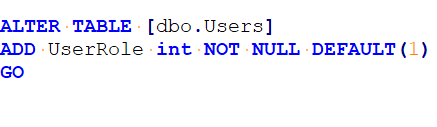
\includegraphics[width=0.5\textwidth]{adduserrole}
    \caption{Rozdielový SQL skript}
    \label{fig:mesh1}
\end{figure}

V tomto prípade sme zo všetkých uživateľov spravili administratorov. Postupne sme prešli jednotlivé záznamy a upravili skupinu podľa konkrétnych užívateľov. Pri vytvárani nových užívateľov má administrátor odteraz možnosť zvoliť skupinu novému užívateľovi.\\ Ďalšou časťou bolo prejsť všetky stránky a upraviť  niektoré časti kódu podľa skupiny prihláseného užívateľa. Mojim riešením bolo do každého modelu, ktorý sa vytvára v kontroleri a zobrazuje na stránke, pridať ďalšiu premennú, ktorú naplním užívateľovou skupinou. Tu dokážem zistiť vytiahnutím aktuálne prihláseného uživateľa z DBContextu, čo je brána, ktorá slúží na prístup a prácu s databázou. Na jednotlivých sránkach pomocou napneného modelu  a razora vieme definovať , čo sa má ktorému užívatešovi zobrazovať a čo nie. Operácie ako upravovanie a mazanie môže robiť iba administrátor, v našom prípade užívateľská rola 1. 
\lstset{language=HTML5}
\begin{lstlisting}
<div class="buttonsPanel">
    @if(model.userRole == 1) {
    <div class="editedButtons">
        <img class="edit" src="@Url.Content(" ~/Content/Images/edit.png ")"
         onclick="boardmanage('@(b.Id)')" title="@Locale.GetLocaleString("
            edit ")" />

        <img class="delete" src="@Url.Content(" ~/Content/Images/remove.png ")"
         onclick="deleteBoard(@(b.Id))" title="@Locale.GetLocaleString("
            delete ")"/>
    </div>
    }
</div>\end{lstlisting}
\begin{figure}[h]
    \centering
    
\includegraphics[width=0.001\textwidth]{empty}
    \caption{Zobrazenie operácii pre administrátora}
    \label{fig:mesh1}
\end{figure}
\subsection*{Import udalosti do databázy}
\textit{Zadanie:}\\
Pridať možnosť importu udalostí priamo do databázy z xlsx súboru. Pridať  chybové hlásenia pri  nesprávnom formáte dokumentu a informovať používateľa o výsledku importu
\\\textit{Analýza}\\
Pri niektorých zakazníkoch sme sa streli so zaujímavou požiadavkou. Pre rýchlejšie vkladanie  udalostí na jednotlivé panely by privítali možnosť nadefinovať si ich   v tabuľkovom editore (napr. Excel) a jednoduchým spôsobom vložiť do systému. Takéto riešenie ušetrí veľa času používateľa obzvlášť pri vysokých počtoch stránok a udalostí. Zároveň pridáva možnosť  do budúcnosti vytvoriť aj export udalostí, čo by znamenalo  jednoduchý a rýchly presun z jedného systému do druhého bez zásahu administrátora alebo manuálneho vytvárania.
\\\textit{Riešenie}\\
\section{LightNet TK}
Na projekte LightNet TK som pracoval dokopy približne  30 dní. V tejto dobe  je zahrnutých aj 5 dní učenia  sa architektúry použitej vo frameworku Angular. Jednalo sa najmä o konečnú a finálnu úpravu produktu podľa potrieb zákazníka. Moja práca spočívala v úprave a vytváraní  komponentov napísaných v Typescripte a v malej miere aj práca na API  v jazyku Java s použitím technológie Spring Boot. Vďaka použitiu material design aplikácia vyzerá moderne a prehľadne.
\subsection*{Pridanie šablón pre merania na rozvádzačoch }
\textit{Zadanie:}\\
Pridať do projektu grafy  z meraní. Pridať možnosť zobraziť/schovať jednotlivé inštancie  z meraní. Konečný stav môže užívateľ uložiť ako šablónu.
\\\textit{Analýza:}\\
 Nakoľko sa na tejto stránke nachádzajú 4 grafy  a vysoký počet inštancii v samotných grafoch, je pre úžívateľa pomerne zložité sa v tom rýchlo zorientovať. 
Šablóna bude uľahčovať zobrazenie grafov , ale najmä zprehľadní celú stránku od  údajov, ktoré užívateľ nepotrebuje. Táto úloha sa bude riešiť v prezenčnej vrstve - zobrazenie uživateľovi, tlačidlo na pridanie a výber šablóny . Ukladanie jednotlivých šablón bude prebiehať  na serveri, do Postre SQL databázy.
\\\textit{Riešenie:}\\
Prvým krokom bolo vymyslieť rozmiestnenie jednotlivých  tlačidiel na stránke a realizovať samotný výber šablón. To som realizoval pomocou klasického dropdown listu. V angulare môžeme tento  prvok nájsť pod názvom \textsf{<mat-select>}. V dropdowne budu zobrazené šablóny stiahnuté zo servera. Pre obmedzené miesto vo widgete grafov som sa rozhodol umiestniť tlačidlona pridanie šablóny priamo do dropdown listu. Po výbere tejto možnosti sa zobrazí dialóg pre zadanie názvu šablóny. Tento dialog je realizovaný ako samotný komponent s názvom  \textsf{MatDialog}. Po zadaní názvu sa kontroluje, či užívateľ nezadal nebezpečné symboly ako úvodzovky, pomlčký, medzeru  a podobne. V  tomto zozname tiež bude možnosť pre všetky grafy a inštancie bez možnosti editácie. To je vhodné vtedy, ak úžívateľ chce mať pri vstupe na stránku zobrazené všetky údaje. 
\subsection*{Lokalizácia SK/EN}
\textit{Zadanie:}\\
Lokalizovať aplikáciu do SK/EN jazyka s možnosťou výberu jazyka.
\\\textit{Analýza:}\\
Hlavnou myšlienkou lokalizácie bolo určiť, či sa bude vykonávať na serveri, alebo na strane klienta.
\\\textit{Riešenie:}\\
a
\subsection*{Pridanie kontaktného formuláru }
\textit{Zadanie:}\\
Pridať komponent pre kontaktný formulár. Vytvoriť emailové konto a správne ho nakonfigurovať v aplikácii.
\\\textit{Analýza:}\\
Táto úloha sa dala rozdeliť zase do 2 samostatných úloh. Jednalo sa o vytvorenie formuláru, ktorý vidí užvateľ a  samostatné odoslanie emailu z hrubého klienta na adresu zadanú zákazníkom. Aby aplikácia bola schopná posielať emaily, bolo potrebné vytvoriť emailový učeť a správne ho nakonfigurovať.
\\\textit{Riešenie:}\\
Samostatný formulár sa skladá zo 6 polí(Meno odosielateľa,Spoločnosť, Adresa, Telefón, Email a Text správy) Tieto polia boli vyžiadané zakazníkom  pričom povinne vyplnené polia musia byť Meno, Email a Text správy. V angulári som si vytvoril triedu [meno], ktorá obsahovala všetky polia formuláru. Anglular obsahuje aj knižnice a mechanizmy na prácu s formulármi a ich validaciu Túto knižnicu some si museli naimportovať z  \textsf{cesta///}. Pomocou two-way databinding som načítal dáta  do inštancie tejto triedy. Potrebné validácie a pravidlá sa dajú riešiť dvomi spôsobmi. 
\begin{enumerate}
\item\textbf{Template-driven validácia} Do HTML časti  sa integrujú  atributy pre validáciu vstupov napr.: \textsf{required, minlenght, maxlenght}. Takýmto spôsobom  je niej možné formulár validovať dynamicky, čo v našom prípade ani nepotrebujeme.
\item\textbf{Reactive form validácia} Pod týmto názvom sa skrýva komplexnejšia  validácia v angular aplikáciách. Validácia sa vytvára priamo v triede komponentu pomocou funkcii.  Toto je vhodné, ak chceme validovať nejaké polia dynamicky, napríklad kontrolovať, či sa zadaná emailová adresa  už nieje použitá bez odoslania formuláru.
 V našom  prípade som sa rozhodol použiť Template-driven validáciu nakoľko postačuje pre náš kontaktný formulár. 

\end{enumerate} 
 Druhou časťou bolo nájsť možnosť, ako posielať správy na email zakazníka. Bolo potrebne vytvoriť prostredníka, ktorý údaje z formuláru prepošle na email.  Ja som sa rozhodol vytvoriť emailovú schránku a nakonfigurovať ju v serverovej časti.
\subsection*{Optimalizácia pre mobilné zariadenia}
\textit{Zadanie:}\\
Optimalizovať aplikáciu pre všetky mobilné zariadenia a bežne používané prehliadače.
\\\textit{Analýza:}\\
Responzivita webových stránok patrí v roku 2018 už k štandardom a moderný web sa bez nej nezaobíde. Minimálne rozlíšenie, na ktoré som sa rozhodol aplikáciu optimalizovať  bolo na šírku  350px, čo zvládné väčšina súčasných mobilných telefónov.  Samotné rozloženie  informácii z aplikácie je rozdelené to tzv. widgetov čo predstavovalo okno s plávajúcou šírkou podľa obsahu. Ďalšou úlohou bude upraviť  texty aj v hornej lište, pretože obsahuje veľký počet informácii (čas, meno prihláseného užívateľa, výber jazyka, odhlásenie)
\\\textit{Riešenie:}\\
Samotnú responzivitu som riešil  úpravou CSS tried pomocou \textsf{@media-query}, čo je funkcia, ktorá sa používa v CSS3. V nej sa zadefinuje pomocou parametrov, či chceme zmeniť triedu keď je rozlíšenie väčšie alebo menšie ako zadané v parametri. Ja som sa rozhodol upravovať triedy pre 3 rôyne rozlíšenia:
\begin{enumerate}
\item \textbf{350px- ???px} - Rozlíšenie, ktoré je možné nájsť na väčšine mobilných telefónov.
\item \textbf{???p - ??? px} -  Rozlíšenie, ktoré sa používa na tabletoch, poprípade na mobilných telefónoch otočených horizontálne (na šírku)
\item \textbf{>??px} -  Rozlíšenie použité na notebokoch a stolových počítačoch. Na tejto sekcii bolo vykonaných najmenej úprav, keďže stránka bola vyvíjaná na notebooku s takýmto rozlíšením.
\end{enumerate}
Responzivitu môžeme jednoducho simulovať použitým vývojárskych nástrojov  v google Chrome.  Po 
\subsection*{Inteligentná lišta }
\textit{Zadanie:}\\
Pridať navigačnú lištu s tlačidlami a aktualnym časom. Lišta sa po posune stránky nadol skryje a po posune stránky hore sa opäť zobrazí.
\\\textit{Analýza:}\\
Inteligentnú lištu môžeme nájsť na takmer každej modernej webovej stránke. Jej úlohou je najmä zväčšiť plochu užitočných informácii na stránke, ale stále mať k dispozicii dôležité odkazy a tlačidlá  bez  zbytočného scrollovania na vrch stránky. Veľž rozdiel je spoznatelný najmä pri prehliadaní stránky na mobilnom zariadení s malým rozlíšením. 
\\\textit{Riešenie:}\\
Pre túto úlohu bolo potrebné upraviť komponent \textsf{<mat-toolbar>}. Nakoľko originálny komponent neposkytuje možnosť samoschovávania lišty, bolo potrebné ju naimplementovať. Pre úpravu html komponentov používam CSS3.Zároveň bolo potrebné detekovať užívateľov pohyb na stránke nahor a nadol pre zobrazenie a skrytie lišty. To som  urobil pomocou registrácie listenera priamo v hlavnom komponente.  Pre krajší efekt a lepší UX  zážitok  som okrem posunu lišty a jej skrytia pridal atribut na zníženie priehľadnosti \textsf{opacity:0}

\section{Správa operátoro??v}
xxx je jeden z prvých projektov, ktorý beží na našej novej propietárne vyvinutej platforme, s čím súviselo aj súčasné odlaďovanie chýb na platforme. Jedná sa o ASP.NET webove stránky napísané v jazyku C\#. Ako ORM nástroj  bol použitý Entity framework. Projekt je vyvíjaný podľa architektúry MVC, ktorá oddeluje rôzne vrstvy systému. Súčasne s MVC architekrúrou boli použité aj ďalšie návrhové vzory. Pre oddelenie business logiky od kontrolerov a pre prácu s DB je použitý návrhový vzor \textbf{Repozitár}. V projekte je vytvorený repozitár pre každú entitu  čím  sprehľadnuje celú aplikáciu a sústreduje všetky metody na prístup do databázy na jedno miesto. Ďalší návrhový vzor je \textbf{Unit OF Work}. Ten sa stará o 


\newpage	

%\backmatter

\thispagestyle{empty}
\nocite{*}
\clearpage

\printbibliography

\end{document}


